\begin{enumerate}
\textbf{NOTE:  YOU MUST HAVE PYTHON3 ENABLED IN ORDER TO RUN THIS. PLEASE TYPE THE FOLLOWING COMMAND:}
\begin{verbatim}
    source /opt/rh/python33/enable
\end{verbatim}

    \item Step by step running
        \begin{itemize}
            \item Open up a terminal in Linux with the project downloaded.
            \item Change your working directory to \begin{verbatim}/http_server/python \end{verbatim}
            \item Type the following command: \begin{verbatim} sh run.sh \end{verbatim}
            \item In your web browser, type the following into your web address bar: \begin{verbatim} localhost:28961 \end{verbatim}
            \item You are now on the web server's index.html page.
           \end{itemize}
    \item screenshot of run command 
    \begin{figure}[!htbp]
  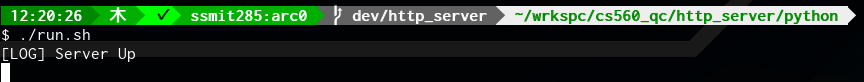
\includegraphics[width=\textwidth]{screenrun.png}
  \caption{The figure above shows the run command to start the web server and the result of the webserver running.}
\end{figure}
\FloatBarrier
\end{enumerate}